% PortfolioOpt.jl: how a portfolio problem is put together.
%
% Three independent choices (a model of the returns, a measure of the portfolio
% return, and the role the measure plays) make one portfolio problem; each measure
% enters the JuMP model through a conic representation, so any conic solver gives
% the decision w*. A walk-forward backtest repeats this on rolling windows.
% Notation follows docs/src/theory/problem.md.
%
% Build: make -C docs/src/assets/diagrams/src
%   pdflatex formulation.tex                                    -> wide layout
%   pdflatex -jobname=portfolioopt--formulation-compact formulation.tex -> narrow layout
\documentclass[tikz,border=4pt]{standalone}
\usepackage{amsmath,amssymb,bm}
\usepackage[T1]{fontenc}
\usepackage[scaled=0.92]{helvet}
\renewcommand{\familydefault}{\sfdefault}
\usetikzlibrary{arrows.meta,shapes.geometric,shapes.symbols,calc,positioning}

% palette of the TS-DDR figure
\definecolor{dTeal}{HTML}{1A9AA0}
\definecolor{dTealLine}{HTML}{3FB3B8}
\definecolor{dNavy}{HTML}{3F4C8C}
\definecolor{dInk}{HTML}{1E2235}
\definecolor{dRed}{HTML}{E4573D}
\definecolor{dCoral}{HTML}{E2765A}
\definecolor{dOrange}{HTML}{F4A93B}
\definecolor{dPeach}{HTML}{FBD9AC}
\definecolor{dPanel}{HTML}{EEF0F2}
\definecolor{dGray}{HTML}{8A90A0}
\definecolor{dShadow}{HTML}{D5DAE3}

\newif\ifcompact
\edef\compactname{\detokenize{portfolioopt--formulation-compact}}
\edef\jobstr{\jobname}
\ifx\jobstr\compactname\compacttrue\fi

\tikzset{
  >={Stealth[length=5pt,width=4pt]},
  every node/.style={text=dInk},
  title/.style={anchor=west,font=\normalsize,inner sep=0pt},
  head/.style={font=\normalsize\bfseries,text=dNavy},
  note/.style={font=\itshape\small,text=dNavy},
  dia/.style={diamond,fill=dOrange,draw=none,minimum size=0.95cm,inner sep=0pt,aspect=1,
              font=\normalsize},
  card/.style={rectangle,rounded corners=4pt,fill=white,draw=dShadow,line width=0.6pt},
  chip/.style={rectangle,rounded corners=3pt,fill=dPanel,draw=none,font=\normalsize,
               inner xsep=4pt,inner ysep=3pt,anchor=west},
  fwd/.style={->,dTealLine,line width=0.9pt},
  wout/.style={->,dOrange,line width=0.9pt},
}

% Lane frame in the paper style: two shadow copies behind a teal rounded frame.
\newcommand{\lane}[4]{% #1 x0, #2 y0, #3 x1, #4 y1
  \foreach \o/\c in {0.16/dShadow!60,0.08/dShadow}
    \draw[\c,fill=white,rounded corners=5pt,line width=0.6pt]
      (#1+\o,#2-\o) rectangle (#3+\o,#4-\o);
  \draw[dTealLine,fill=white,rounded corners=5pt,line width=0.9pt] (#1,#2) rectangle (#3,#4);}

% Glyphs for the three kinds of returns model, centred at #1.
\newcommand{\glyphP}[1]{\begin{scope}[shift={(#1)}]
  \fill[dPeach] plot[domain=-0.45:0.45,samples=30] (\x,{0.34*exp(-18*\x*\x)}) -- (0.45,0) -- (-0.45,0) -- cycle;
  \draw[dOrange,line width=0.7pt] plot[domain=-0.45:0.45,samples=30] (\x,{0.34*exp(-18*\x*\x)});
  \draw[dGray,line width=0.4pt] (-0.5,0) -- (0.5,0);\end{scope}}
\newcommand{\glyphS}[1]{\begin{scope}[shift={(#1)}]
  \foreach \x/\y in {-0.38/0.10,-0.22/0.28,-0.05/0.05,0.08/0.22,0.22/0.12,0.36/0.30,-0.30/0.20,0.30/0.02}
    \fill[dOrange] (\x,\y) circle (0.045);
  \draw[dGray,line width=0.4pt] (-0.5,-0.06) -- (0.5,-0.06);\end{scope}}
\newcommand{\glyphU}[1]{\begin{scope}[shift={(#1)}]
  \draw[dOrange,fill=dPeach,line width=0.7pt,rotate=25] (0,0.15) ellipse (0.42 and 0.2);
  \fill[dInk] (0,0.15) circle (0.04);\end{scope}}

% Column contents (shared by both layouts). #1 = top-left corner of the column.
\newcommand{\returnscol}[1]{\begin{scope}[shift={(#1)}]
  \node[head,anchor=west] at (0,0) {Returns model};
  \glyphP{0.5,-1.0}   \node[anchor=west] at (1.15,-0.8) {$P$};
                      \node[note,anchor=west] at (1.15,-1.2) {distribution};
  \glyphS{0.5,-2.15}  \node[anchor=west] at (1.15,-1.95) {$r_1,\dots,r_S$};
                      \node[note,anchor=west] at (1.15,-2.35) {samples};
  \glyphU{0.5,-3.3}   \node[anchor=west] at (1.15,-3.1) {$\mathcal{P}$};
                      \node[note,anchor=west] at (1.15,-3.5) {ambiguity set};
\end{scope}}
\newcommand{\measurecol}[1]{\begin{scope}[shift={(#1)}]
  \node[head,anchor=west] at (0,0) {Measure $\rho(w)$};
  \node[chip] at (0,-0.8)  {$\mathbb{E}_P[r^\top w]$};
  \node[chip] at (0,-1.5)  {$\lVert \Sigma^{1/2} w\rVert_2$};
  \node[chip] at (0,-2.2)  {$-\mathrm{CVaR}_\alpha(r^\top w)$};
  \node[chip] at (0,-2.9)  {$\min_{P\in\mathcal{P}} \mathbb{E}_P[r^\top w]$};
  \node[note,anchor=west] at (0,-3.5) {\dots\ or your own};
\end{scope}}
\newcommand{\rolecol}[1]{\begin{scope}[shift={(#1)}]
  \node[head,anchor=west] at (0,0) {Role};
  \node[note,anchor=west] at (0,-0.75) {objective term};
  \node[chip] at (0,-1.25) {$c_j\,\rho_j(w)$};
  \node[note,anchor=west] at (0,-2.05) {risk constraint};
  \node[chip] at (0,-2.55) {$\rho_i(w)\in\mathcal{C}_i$};
\end{scope}}

\newcommand{\problem}{%
  $\begin{aligned}
    \max_{w}\;\; & \displaystyle\sum_{j} c_j\,\rho_j(w)\\[2pt]
    \text{s.t.}\;\; & \rho_i(w)\in\mathcal{C}_i, \quad i=1,\dots,m\\[2pt]
    & w\in\mathcal{X}
  \end{aligned}$}
\newcommand{\conic}{%
  $\rho(w)\;\to\; f(w,u),\;\; (w,u)\in\mathcal{K}$}

\begin{document}
\ifcompact
% ============================ narrow (phone) layout ============================
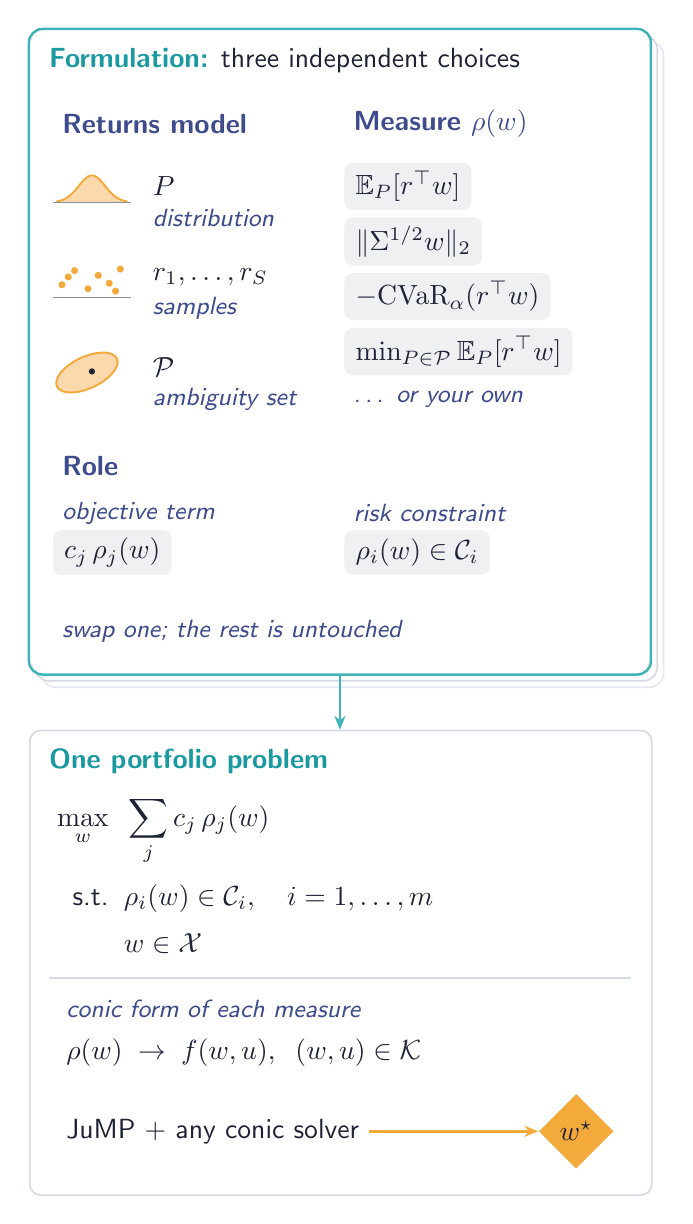
\begin{tikzpicture}
  \lane{0}{6.4}{7.9}{14.6}
  \node[title] at (0.25,14.2) {\textcolor{dTeal}{\bfseries Formulation:} three independent choices};
  \returnscol{0.3,13.4}
  \measurecol{4.0,13.4}
  \node[head,anchor=west] at (0.3,9.05) {Role};
  \node[note,anchor=west] at (0.3,8.45) {objective term};
  \node[chip] at (0.3,7.95) {$c_j\,\rho_j(w)$};
  \node[note,anchor=west] at (4.0,8.45) {risk constraint};
  \node[chip] at (4.0,7.95) {$\rho_i(w)\in\mathcal{C}_i$};
  \node[note,anchor=west] at (0.3,6.95) {swap one; the rest is untouched};
  \node[card,minimum width=7.9cm,minimum height=5.9cm,anchor=north west] (pb) at (0,5.7) {};
  \draw[fwd] (3.95,6.4) -- (3.95,5.7);
  \node[title] at (0.25,5.3) {\textcolor{dTeal}{\bfseries One portfolio problem}};
  \node[anchor=north west,inner sep=0pt] at (0.35,4.85) {\problem};
  \draw[dShadow,line width=0.6pt] (0.25,2.55) -- (7.65,2.55);
  \node[note,anchor=west] at (0.35,2.15) {conic form of each measure};
  \node[anchor=west] at (0.35,1.6) {\conic};
  \node[anchor=west] (jump) at (0.35,0.6) {JuMP + any conic solver};
  \node[dia] (w) at (6.95,0.6) {$w^\star$};
  \draw[wout] (jump.east) -- (w.west);
\end{tikzpicture}
\else
% =============================== wide layout ===================================
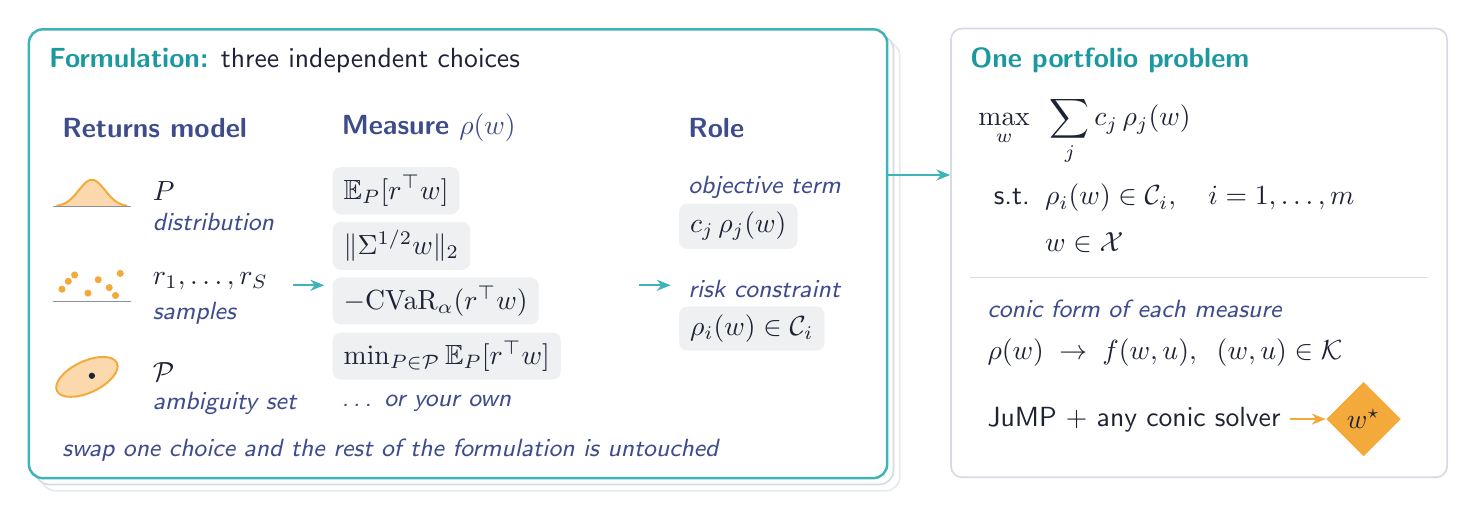
\begin{tikzpicture}
  \lane{0}{0}{10.9}{5.7}
  \node[title] at (0.25,5.3) {\textcolor{dTeal}{\bfseries Formulation:} \textcolor{dInk}{three independent choices}};
  \returnscol{0.3,4.45}
  \measurecol{3.85,4.45}
  \rolecol{8.25,4.45}
  \draw[fwd] (3.35,2.45) -- (3.75,2.45);
  \draw[fwd] (7.75,2.45) -- (8.15,2.45);
  \node[note,anchor=west] at (0.3,0.35) {swap one choice and the rest of the formulation is untouched};

  \node[card,minimum width=6.3cm,minimum height=5.7cm,anchor=south west] (pb) at (11.7,0) {};
  \node[title] at (11.95,5.3) {\textcolor{dTeal}{\bfseries One portfolio problem}};
  \node[anchor=north west,inner sep=0pt] at (12.05,4.85) {\problem};
  \draw[dShadow,line width=0.6pt] (11.95,2.55) -- (17.75,2.55);
  \node[note,anchor=west] at (12.05,2.15) {conic form of each measure};
  \node[anchor=west] at (12.05,1.6) {\conic};
  \node[anchor=west] (jump) at (12.05,0.75) {JuMP + any conic solver};
  \draw[fwd] (10.9,3.85) -- (11.7,3.85);
  \node[dia] (w) at (16.95,0.75) {$w^\star$};
  \draw[wout] (jump.east) -- (w.west);
\end{tikzpicture}
\fi
\end{document}
